\documentclass[submit,techreq,noauthor]{eco}	% semi style
\usepackage[dvips]{graphicx}
\usepackage{listings, jlisting} 		% for source code
\usepackage{url}
\usepackage{setspace}
\usepackage{here}
%\setstretch{1.5} % 行間を広くします(資料チェックしてもらうときはコメントを外す)

\lstset{
  basicstyle={\ttfamily},
  identifierstyle={\small},
  commentstyle={\smallitshape},
  keywordstyle={\small\bfseries},
  ndkeywordstyle={\small},
  stringstyle={\small\ttfamily},
  frame={tb},
  breaklines=true,
  columns=[l]{fullflexible},
  numbers=left,
  xrightmargin=0zw,
  xleftmargin=3zw,
  numberstyle={\scriptsize},
  stepnumber=1,
  numbersep=1zw,
  lineskip=-0.5ex
}

\begin{document}

\semino {5/18}					% 年度/回数
\date   {5/05/26/水}				% 平成/月/日/曜日
\title  {ライブラリ関数単位でのプログラムへの影響と\\システムコールの比較}	% タイトル
\author {奥 若菜}				% 氏名


\begin{abstract}
	Linuxマシンが製品やサービスの基盤として広く利用されるようになっていることで,それを標的とするLinuxマルウェアが劇的に増加している.
  また,Linuxマルウェアの開発動向として,マルウェアが自身の攻撃をセキュリティソフトに検知されないようにする回避技術の大幅な向上が確認されている.
  2021年に発見されたマルウェアSymbioteは,一般的に見られるLinuxマルウェアと比較して,極めて検出が困難とされる.
  SymbioteはLD\_PRELOADを使用して,すべての実行中のプロセスにロードされる共有ライブラリとして動作し,
  正当なプロセスの下で自身や他のマルウェアの痕跡を隠蔽する.
  本研究では,Symbioteのような,共有ライブラリを用いた攻撃を行うマルウェアを動的解析し,その挙動を明らかにするとともに,効果的な検知手法の発見を目指す.
  はじめに,Symbioteを静的解析することで,エクスポートされるライブラリ関数の役割や隠蔽されるファイル名・プロセス名を特定した.
  前回から今回では,Symbioteのライブラリ関数を使用するプログラムを実行したときの実行結果とシステムコールの差分を収集する.
\end{abstract}
\maketitle


\section{はじめに}
IoTデバイスの普及や企業のクラウドシフトにより,製品やサービスの基盤として,Linuxマシンを利用するケースが増えた.
攻撃対象が広がったことで,それを標的とするLinuxマルウェアも劇的に増加している\cite{TREND-MICRO}.
Linuxマルウェアの開発動向としては,マルウェアが自身の攻撃をセキュリティソフトに検知されないようにする回避技術の大幅な向上が確認されている\cite{IBM}.
%Linuxマルウェアの技術革新の水準はWindowsベースのマルウェアに迫る勢いとされ,この傾向は2022も高まると予想されている.
このことから,今後もより高度な潜伏機能を持つマルウェアが開発される可能性が高く,対策を怠ると重大な被害に繋がると考えられる.\cite{A}


2021年に発見されたSymbioteは,Linuxで一般的に見られるマルウェアとは異なる特徴を持ち,極めて検出が困難とされる\cite{Symbiote}.
Symbioteは,単独の実行可能ファイルではなく,LD\_PRELOADによってすべての実行中のプロセスにロードされる共有ライブラリとして動作する.
LD\_PRELOADとは,Linuxにおいて,プログラム実行時に共有ライブラリを動的リンクするために使用される環境変数である.
Symbioteは,LD\_PRELOADを使用することで,プログラムによって要求される正当な共有ライブラリの代わりに,悪意のある共有ライブラリを提供する.
このように悪意のある共有ライブラリをプログラムにロードし,不正なコードを実行する攻撃をDynamic Linker Hijackingという\cite{MITRE-ATT&CK}.
この攻撃では正当なプロセスの下で,注入されたコードの実行が隠されるため,プロセスベースの解析は回避される可能性が高い.

本研究は,動的解析を行うことによってSymbioteの挙動を明らかにすることを目指す.
また,SymbioteのようなDynamic Linker Hijackingを行うLinuxマルウェアの効果的な検知手法および対策方法を考察する.


以下,2章でSymbioteの機能を説明し,3章で静的解析によって得られた検体の詳細な設計を説明する.
4章で検体を用いた動的解析の結果を述べ,5章でまとめる.\\


\section{Symbioteの機能}
Symbioteが初めて検知されたのは2021年11月であり,
ラテンアメリカの金融セクターを標的とするために作成されたとされている.
Symbioteについての調査は,Intezerの研究者Joakim KennedyとBlackBerryのResearch and Intelligence Teamによって
行われ,レポートが作成されている.以下に文献\cite{Symbiote}のレポートをもとにSymbioteの機能を示す.


\subsection{検知回避機能}
Symbioteは,LD\_PRELOADで指定した共有ライブラリによって,プログラムによる関数の呼び出しをフックし,
悪意のあるコードを実行することで,検知を回避する.具体的には,C言語の標準ライブラリであるlibcおよび
パケットキャプチャのためのライブラリであるlibpcapの関数をフックすることで,以下のような回避機能を実現する.
  \begin{description}
    \item [プロセスの隠蔽] \mbox{}\\
    呼出し元のアプリが/proc以下にあるファイルまたはディレクトリにアクセス
    しようとすると,プロセス名を元に出力を消去する.
    \item [ファイルの隠蔽] \mbox{}\\
    呼出し元のアプリが上記以外の場所にアクセスしようとすると,暗号化さ
    れたファイルリストにある名前を元に出力を消去する.
    \item [ネットワークトラヒックの隠蔽] \mbox{}
      \begin{description}
        \item[UDP:] 
        libpcapライブラリの関数をフックし,受信したパケットごとにドメインの文字列をチェックする.一致した場合はそのパケットをスキップして呼出し元に返す.
        \item[TCP:] 
        fopenとfopen64をフックし,プロセスがproc/net/tcpを開こうとすると,該当するポートをスキップして呼出し元に返す.
        感染マシンがeBPFを使用してパケットキャプチャを行う場合は,setsockoptをフックし,提供されたeBPFコードの前に独自のバイトコードを付加することで,ポートに基づきパケットを消去する.
      \end{description}
  \end{description}

\subsection{ルートキット機能}
Symbioteはすべての実行中のプロセスに感染した後,認証情報を収集し,攻撃者にリモートアクセスなどのルートキット機能を提供する.

認証情報の収集は,sshやscpプロセスによって呼び出されるlibcのread関数をフックすることで行われる.
収集した認証情報はファイルに書き込まれるだけでなく,
16進エンコードされ,攻撃者が運用するサーバにDNSのAレコード要求を通じて持ち出される.\\
\indent
感染したマシンへのリモートアクセスは,Pluggable Authentication
Module(PAM)機能をフックすることで提供される.アプリケーション(telnetやssh)がPAMを利用してユーザを認証する際に,攻撃者のあら
かじめ設定したものと同じ認証情報でアクセスすると,フックされた関数が成功応答を返すとともに,攻撃者もアクセスが可能になる.

\subsection{緊急アクセス機能}
Symbioteは通常のプロセスが機能しない場合に,攻撃者のC\&CサーバにDNSのTXTレコード要求を送信し,マシンへの緊急アクセスを
提供する.TXTレコードの形式は,\%MACHINEID\%.\%C\&C\_DOMAIN\%となっている.応答を取得すると,このマルウェアはコンテンツをbase64
デコードし,コンテンツが正しいed25519秘密鍵で署名されているかどうかをチェックし,
RC4でコンテンツを復号して,生成されたbashプロセスでシェルスクリプトを実行する.\\


\section{静的解析によるSymbioteの調査}
2章では,文献\cite{Symbiote}のレポートで示されているSymbioteの機能を紹介した.
ただし,このレポートはSymbioteで一般的に見られる機能を紹介しており,具体的な検体の情報は明記されていない.
また,その他の文献についても,検体ごとの詳細な情報を示すものは見つかっていない.
\indent
Symbioteでは,複数の検体において類似した機能が見られることが示されているが,検体が提供するライブラリ関数や,隠蔽されるファイル・プロセスの名前はそれぞれの検体で異なる.
Symbioteのそれぞれの検体について静的解析を行い,詳細な設計を明らかにする.

\subsection{検体}
マルウェア分析プラットフォームであるIntezer AnalyzeとVirusTotalを用いてSymbioteを探索したところ,表\ref{table: Artifact}に示す6検体が見つかった.
これらはIntezerのレポートに記載されている検体のハッシュと一致しており,更新情報もないため,現在まででSymbioteとされている検体は,この6検体が全てである可能性が高い.\\
アップロード日の項目には,Intezer Analyzeへ検体がアップロードされた日付を示す.ファイル名の項目には,攻撃者によって検体ファイルに設定されると想定される名前を示す.
また,ライブラリ関数の項目には検体の共有ライブラリによってエクスポートされる関数の数を示す.\\
\indent
6検体のうち,検体4のみが実行ファイルであり,実行を開始すると2.3節で述べた緊急アクセス機能を提供する.
その他の検体は,すべて共有ライブラリファイルであり,LD\_PRELOADに検体ファイルのパスを設定することで動作する.

\subsection{検体によってエクスポートされるライブラリ関数}
Symbioteの共有ライブラリはELFファイルであるため,readelfコマンドを用いてライブラリ関数のシンボル情報を
取得できる.表2は,Symbioteの5つの共有ライブラリについて,エクスポートされるライブラリ関数の一覧を示す.丸がついているライブラリ関数は,その検体からエクスポートされることを表している.
検体間でエクスポートされるライブラリ関数がほとんど共通していることから,それぞれの共有ライブラリは,バージョン違いの検体であると分か
る.


\begin{table*}[t]
  \caption{Symbioteの検体とファイル名一覧}
  \label{table: Artifact}
  \centering
  \begin{tabular}{|c|c|c|c|}
  \hline
  No. & hash256                                                                                                        & アップロード日 & ファイル名 \\ \hline
  1   & \begin{tabular}[c]{@{}l@{}}121157e0fcb728eb8a23b55457e89d45\\ d76aa3b7d01d3d49105890a00662c924\end{tabular} & 2021/11/27 & kerneldev.so \\ \hline
  2   & \begin{tabular}[c]{@{}l@{}}f55af21f69a183fb8550ac60f392b05d\\ f14aa01d7ffe9f28bc48a118dc110b4c\end{tabular} & 2022/01/19 & mt64.so \\\hline
  3   & \begin{tabular}[c]{@{}l@{}}ec67bbdf55d3679fca72d3c814186ff4\\ 646dd779a862999c82c6faa8e6615180\end{tabular} & 2022/01/26 & search.so \\ \hline
  4   & \begin{tabular}[c]{@{}l@{}}45eacba032367db7f3b031e5d9df10b\\ 30d01664f24da6847322f6af1fd8e7f01\end{tabular} & 2022/01/29 & dnscat\\ \hline
  5   & \begin{tabular}[c]{@{}l@{}}a0cd554c35dee3fed3d1607dc18debd\\ 1296faaee29b5bd77ff83ab6956a6f9d6\end{tabular} & 2022/02/01 & liblinux.so \\ \hline
  6   & \begin{tabular}[c]{@{}l@{}}cb4bbe3af754779e673c6ae84cb38d7f\\ 2ccbc9a1d59c52abbb98451d070dba3c\end{tabular} & 2022/08/19 & libpcap3.so \\ \hline
  \end{tabular}
\end{table*}


\begin{table*}[t]
  \caption{エクスポートされるライブラリ関数一覧}
  \label{table: library}
  \centering
  \begin{tabular}{|c|c|c|c|c|c|}
  \hline
  ライブラリ関数           & kerneldev.so & mt64.so & search.so & liblinux.so & libpcap3.so \\ \hline
  \_fini            & ○            & ○       & ○         & ○           & ○           \\ \hline
  \_init            & ○            & ○       & ○         & ○           & ○           \\ \hline
  fopen,fopen64     & ○            & ○       & ○         & ○           & ○           \\ \hline
  readdir,readdir64 & ○            & ○       & ○         & ○           & ○           \\ \hline
  fstatat,fstatat64 &              & ○       & ○         & ○           & ○           \\ \hline
  pam\_set\_item    & ○            & ○       & ○         & ○           & ○           \\ \hline
  pam\_acct\_mgmt   &              & ○       & ○         & ○           & ○           \\ \hline
  pam\_authenticate & ○            & ○       & ○         & ○           & ○           \\ \hline
  crc32b            & ○            &         &           &             &             \\ \hline
  RC4               & ○            &         &           &             &             \\ \hline
  recvmsg           &              & ○       & ○         & ○           & ○           \\ \hline
  pcap\_stats       &              & ○       & ○         & ○           & ○           \\ \hline
  pcap\_loop        &              & ○       & ○         & ○           & ○           \\ \hline
  setsockopt        &              & ○       & ○         & ○           & ○           \\ \hline
  download\_script  &              &         & ○         & ○           &             \\ \hline
  prepare\_pipe     &              &         & ○         & ○           &             \\ \hline
  read              & ○            & ○       & ○         & ○           & ○           \\ \hline
  execve            &              & ○       & ○         & ○           &             \\ \hline
  stat              &              & ○       & ○         & ○           & ○           \\ \hline
  statx             &              & ○       & ○         & ○           & ○           \\ \hline
  \end{tabular}
  \end{table*}

\subsection{検体1(kerneldev.so)の解析結果}
実行中のプロセスに提供されるライブラリ関数と,それらの呼出し関係に注目して,検体1の静的解析を行った.
現時点では検体1のみの結果を示すが,検体1では実装されていないライブラリ関数の機能も明らかにするために,その他の検体についても今後は静的解析を行う予定である.\\
\subsubsection{ライブラリ関数}
検体1によって提供される13個のライブラリ関数と,その機能を以下にまとめる.
これらの関数は,libcなどのライブラリ関数と同様の機能を提供しつつ,隠蔽や認証情報の収集,攻撃者との通信を行う.
\begin{description}

  \item [プログラムの初期化・終了処理] \mbox{}
  \begin{description}
    \item[\_init:] プログラムの初期化処理を行う.
    \item[\_fini:]プログラムの終了処理を行う.
  \end{description}

  \item [TCP通信・ファイル・プロセスの隠蔽] \mbox{}
  \begin{description}
    \item[fopen・fopen64:] ファイルを開く.隠蔽するポートの内容はファイルに書き込まない.
    \item[readdir・readdir64:] ディレクトリエントリを返す.隠蔽するファイルとプロセスはNULLを返す.
  \end{description}

    \item [認証情報の収集] \mbox{}
  \begin{description}
    \item[pam\_authenticate:] PAMを使用してユーザ認証を行う.ユーザ名やパスワードを収集する.
    \item[pam\_set\_item:] PAM項目の値を更新する.PAM項目がパスワードなら保存する.\\
  \end{description}

  \item [キーロギング・通信・暗号化] \mbox{}
  \begin{description}
    \item[read:] コマンドラインの情報とホストのIPアドレスを収集し,攻撃者に送信する.
    \item[recvmsg:]ソケットからデータを受信する.ポートや文字列に基づいて隠蔽する.
    \item[crc32b:] crc32のハッシュ値を返す.
    \item[RC4:] RC4で文字列の暗号化を行う.\\
  \end{description}
\end{description}

\subsubsection{関数の呼出し関係}
検体1によって実行中のプロセスに提供されるのは3.2.1節で示した13個のライブラリ関数のみである.
しかし,検体の挙動を明らかにするためには,それらのライブラリ関数によって二次的に呼び出される関数も調査する必要がある.\\
\indent
例えば,検体1が提供するreaddirは図\ref{fig:call-graph}のように関数呼出しを行っている.呼出される関数のうち,
check\_proc,hidden\_proc,hidden\_fileは,readdirと同様に検体1によって実装された関数であり,プロセスやファイルの隠蔽のために使用される.
一方で,dlsymとstrcmpはlibcライブラリによって検体の関数に提供され,特にdlsymはlibcで定義される本来のreaddirを呼び出すために使用される.\\


\begin{figure}[t]
	\centering
  \fbox{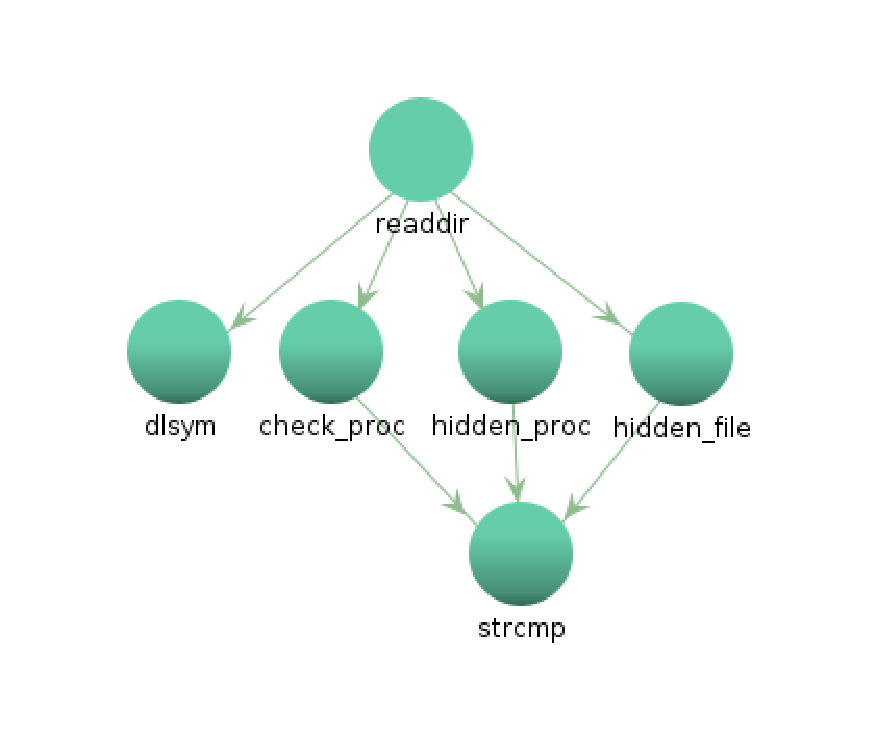
\includegraphics[width=7cm]{fig/call-graph.eps}}
	\caption{readdirの呼出し関係}
	\label{fig:call-graph}
\end{figure}

\subsubsection{隠蔽されるファイル・プロセスの名前}
hidden\_proc,hidden\_fileはプロセスやファイルの隠蔽のために使用される関数である.これらが参照するアドレスを調べることで,
検体1によって隠蔽されるファイル名とプロセス名を特定することができる.以下にそれらを示す.
\begin{description}
  \item[隠蔽されるプロセス] 
  \begin{itemize}
    \item kernelconfig
    \item kerneldev
    \item threadmulti
  \end{itemize}
  \item[隠蔽されるファイル] 
  \begin{itemize}
    \item kernelconfig
    \item kerneldev
    \item threadmulti
    \item usb.h
    \item kerneldev.so \\
  \end{itemize}
\end{description}

\begin{figure*}[t]
	\centering
  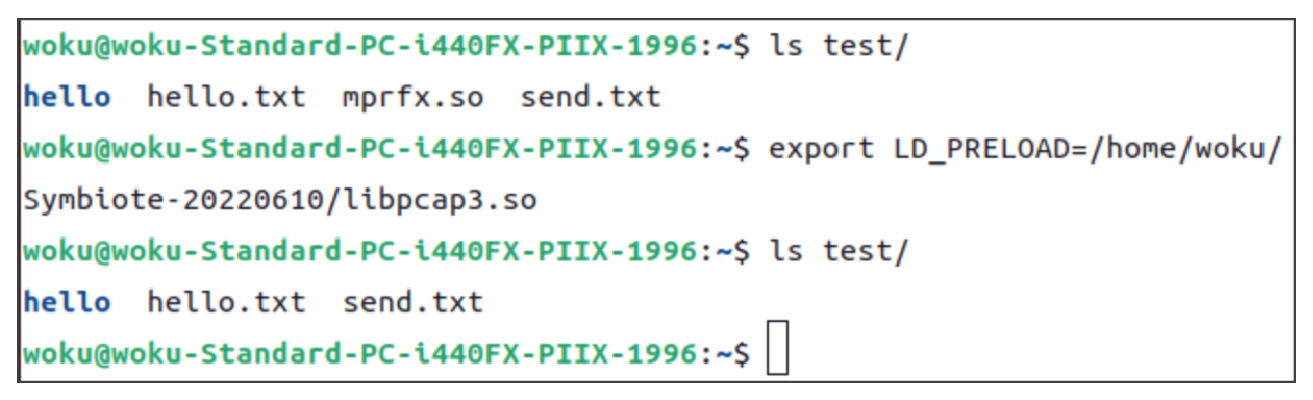
\includegraphics[width=14cm]{fig/ls.eps}
	\caption{lsコマンドの実行結果}
	\label{fig:ls}
\end{figure*}

\section{ライブラリ関数ごとの特徴の収集}
検体を隔離環境で実行し,それぞれのライブラリ関数に対して,それを利用するプログ
ラムを実行したときの出力結果とシステムコールの差分を収集する.今回はreaddirのみについてまとめる.
\indent
4.1節で解析環境について説明し,4.2節でreaddirの調査結果を述べる.

\subsection{解析環境}
解析環境を構成するソフトウェアを表3に示す.
ゲストOSからホストおよびネットワークへのアクセスはできない.
また,検体の実行と解析は全てゲストOS上で行う.



\begin{table}[t]
  \caption{解析環境}
  \label{table: 解析環境}
  \centering
  \begin{tabular}{|l|l|}
  \hline
  Guest OS   & Ubuntu 22.04.2 LTS \\ \hline
  emulator   & QEMU 6.2.0         \\ \hline
  hypervisor & KVM                \\ \hline
  Host OS    & Ubuntu 22.04.2 LTS \\ \hline
  \end{tabular}
\end{table}



\subsection{readdir}
\subsubsection{出力結果}
lsコマンドは内部でreaddirを呼び出す.Symbioteの共有ライブラリを利用する場合としない場合で,lsコマンドを実行したときの出力結果を観測する.
今回lsコマンドには/home以下に存在する/testディレクトリのPATHを指定する./homeの中には/helloディレクトリ,kerneldev.so,send.txt,test.txtが含まれる.
以下のように,Symbioteを設定せずにlsコマンドを実行したあと,検体1(kerneldev.so)をLD\_PRELOADに設定し,再度lsコマンドを実行した.\\
\$ ls /home/.../test/\\
\$ export LD\_PRELOAD=/path/to/kerneldev.so\\
\$ ls /home/.../test/\\
出力結果を図2に示す.通常のreaddirが利用される場合と,検体1のreaddirが利用される場合で,lsコマンドの出力に違いがある.
検体1によって隠蔽されるファイル名と一致しているkerneldev.soは,Symbioteが設定される場合は表示されないことが分かる.\\

\begin{figure*}[t]
	\centering
  \includegraphics[width=15cm]{fig/01.eps}
	\caption{Symbiteなし:ls -aのシステムコール}
	\label{fig:s-ls}
\end{figure*}

\begin{figure*}[t]
	\centering
  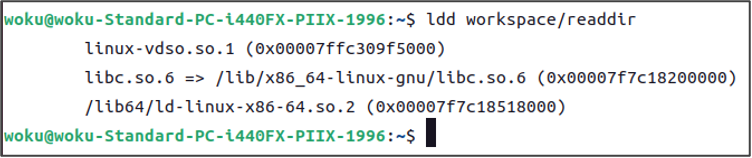
\includegraphics[width=15cm]{fig/02.eps}
	\caption{Symbiteあり(kerneldev.so):ls -aのシステムコール}
	\label{fig:s-ls}
\end{figure*}

\begin{figure}[t]
	\centering
  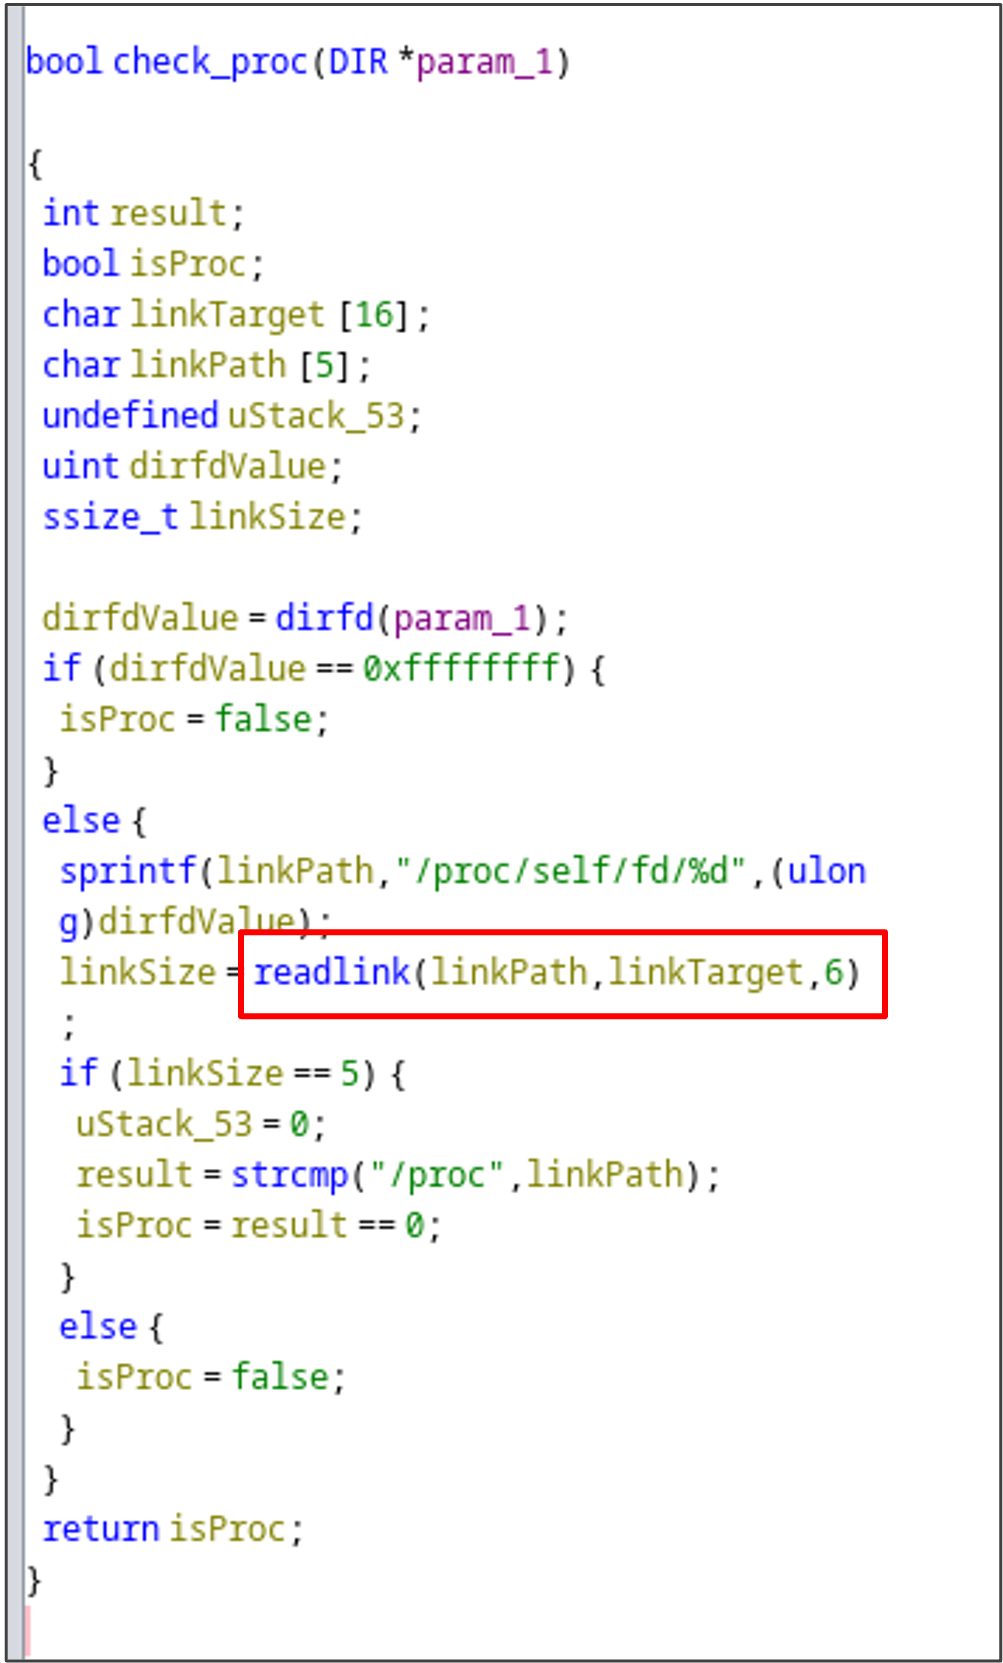
\includegraphics[width=7cm]{fig/07.eps}
	\caption{check\_proc}
	\label{fig:readdir}
\end{figure}

\subsubsection{システムコールトレース}
4.2.1節と同じ条件において,ls -aコマンドを実行したときのシステムコールをstraceで観測する.\\
図3はSymbioteを設定せずにls -aを実行したときのシステムコールの一部,図4はSymbioteを設定してls -aを実行したときのシステムコールの一部である.
これらを比較すると,図3の赤矢印の位置にはないが,図4の対応する位置にはreadlinkシステムコールが全部で6回呼出されていることが分かる. 
readlinkは,与えられたシンボリックリンクから実際のPATHを取得するシステムコールである.システムコールに違いが生じた要因として,
Symbioteによってエクスポートされるreaddirは,内部でcheck\_proc[図5]という関数を呼び出す.check\_procは,指定
されたディレクトリが/proc内のファイルディスクリプタを指すシンボリックリンクであるかを判定するための関数である.
この関数内で,シンボリックリンクから,実際のパスを取得するために,readlinkシステムコールが呼ばれている.
Symbioteが設定されていない場合は,lsコマンドによってreadlinkが呼出されることはないため,特徴的な違いと定義できる可能性がある.\\




\section{おわりに}
LD\_PRELOADを利用することで,共有ライブラリの置き換えを行うLinuxマルウェアである
Symbioteの調査と,その検体の静的解析および動的解析を行った.静的解析をすることで,脅威レポートからは得られなかった検体の詳細な設計を明らかにすることができた.
動的解析では,Symbioteがエクスポートするライブラリに着目して,コマンドの出力結果とstraceの出力結果を取得し,通常時との違いを比較した.
特にreaddirの調査においては,SymbioteはPATHの取得のためにreadlinkシステムコールを呼び出すことがあることを確認できた.\\
今後は,残りのライブラリコールに対しても同様に調査を行っていく.また,並行してライブラリコールの観測からも,Symbiote感染時と
そうでないときで,違いを観測する方法を検討する.

%bibtex
\setlength\baselineskip{12pt}
{\small
	\bibliography{references}
	\bibliographystyle{ipsjunsrt}
}


\end{document}
